\chapter{Experiments}


\section{Introduction}

As we have seen in the previous section, all results of a simulation are stored into several \texttt{.csv} files.

\begin{itemize}
    \item \texttt{states.csv} contains, for each State, its id, population size, VAT rate, levy rate, tariff rate, wealth tax rate, allowance type, unemployment rate, black economy share, GDP, the money it has, the total money of its population (agents), the number of transactions performed by its agents, and the id's of the other States to which it is connected.

    \item \texttt{agents.csv} contains, for each Agent, its id, the id of its State, its initial money (the money with each it started the simulation), its current money, its talent, whether it is a producer or not (thus whether it is employed or unemployed) and the number of purchases it has made.
    
    \item \texttt{products.csv} contains, for each Agent, the id of the Agent producing it, its type, the production price (always set to 0), the selling price, the stock of this product, and the number of sales. Therefore, each agent has one Product and we can merge this file with the agents file.
    
    \item \texttt{ticks.csv} keeps track of different values during the simulation. The following metrics are saved every 100 ticks: the number of ticks that have passed so far, the number of transactions that have happened in the World so far, the total money of all the States, the total money of all the Agents, and the total GDP of all States.
\end{itemize}

Based on these files, we can do various experiments by adjusting the parameters and see the effects on some key metrics. For this, the language Python3 has been chosen as it contains many libraries to analyze and plot such data: pandas, numpy or matplotlib. Rapidness is not the key factor here as the simulation has already stored its results in the \texttt{.csv} files.

The default configuration file that we use is the following. Experiment after experiment, we will modify one or several parameter and see its/their influence. 

\begin{lstlisting}[language=json,firstnumber=1]
{
    "World": {
        "PRODUCT_CHOICE": "CHEAPEST",
        "NB_STATES": 500,
        "NB_AGENTS": 25000,
        "NB_TICKS": 3000,
        "NB_TICKS_SAVE_CSV": 100
    },
    "Connections": {
        "CLUSTER_SIZE": 0,
        "PROB_CONNECTION": 0.0
    },
    "State": {
        "Tax": {
            "MIN_VAT": 0.2,
            "MAX_VAT": 0.2,
            "MIN_LEVY": 0.1,
            "MAX_LEVY": 0.1,
            "MIN_TARIFF": 0.3,
            "MAX_TARIFF": 0.3,
            "VAL_WEALTH_TAX_TOP": 0.1,
            "MIN_WEALTH_TAX_VALUE": 0.2,
            "MAX_WEALTH_TAX_VALUE": 0.2,
            "NB_TICKS_COLLECT_TAXES": 100
        },
        "Allowance": {
            "NB_TICKS_DISTRIBUTE_ALLOWANCES": 100
        },
        "Others": {
            "MIN_UNEMPLOYMENT": 0.05,
            "MAX_UNEMPLOYMENT": 0.05,
            "MIN_BLACK": 0.15,
            "MAX_BLACK": 0.15
        }
    },
    "Agent": {
        "MIN_INIT_MONEY": 1000.0,
        "MAX_INIT_MONEY": 1000.0,
        "RATIO_BUY": 0.5,
        "RATIO_PRODUCE": 0.5
    },
    "Product": {
        "NB_DIFF_PRODUCTS": 50,
        "MIN_PRICE": 0.0,
        "MAX_PRICE": 300.0,
        "MAX_STOCK": 2000
    }
}
\end{lstlisting}

Whenever points are scattered on a plot, we will also plot a line which interpolates, with a degree 2, these points to better highlight the trend. Also, in the bar charts, an average is computed in order to give a global overview. We also have to pay attention that most plots have two $y$ axis (red is for the left hand-side, blue for the right hand-side). There are over 40 plots in the folder \texttt{./report/img/exp/}, we will only focus on the most interesting ones.

For each experiment, we will compare it with the state-of-the-art presented earlier, and try to answers the many research questions introduced in the section~\ref{section:motivation_objectives}.


\section{State experiments}

We will start our experiments with all the parameters related to the State. We should note that to be able to compare fairly different States, the metrics of the State (for instance the total money of its Agents or the GDP) is divided by its population size. 

    \subsection{Experiment 1: No taxes}
    In this first experiment, we will try to see the effects on having no taxes (thus all tax values are set to 0). In the following plots, we will plot the State with regular taxes (as defined earlier) on the left hand-side, and the State with no taxes on the right hand-size. 

        \subsubsection{State GDP and number of transactions}

        We can see on the following plots that a State with no taxes (thus VAT of 0, but the other taxes are also set to 0) will generally have a smaller GDP and the number of transactions is also decreased compared to a State with taxes (left plot where the VAT is 0.2 for instance). 
        
        At first this might seem rather odd since we expect products to be cheaper, therefore more transactions should be happening (hence the GDP would be boosted too). However, if we think more about it, this seems rather logical because a State with no tax will not be able to distribute allowances, and thus some agents will concentrate all the money at the expense of other agents who will not be able to buy products anymore after some time, eventually diminishing both the GDP and the number of transactions.

        \begin{figure}[H]
            \minipage{0.5\textwidth}
                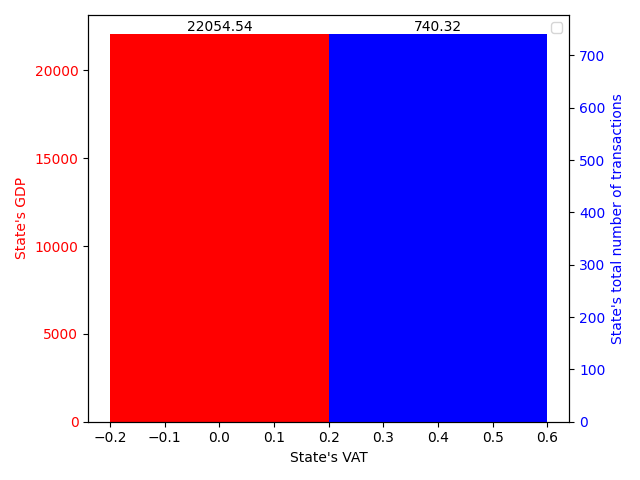
\includegraphics[width=\linewidth]{img/exp/1_1_1.png}
                \caption{Normal taxes (e.g. VAT of 0.2)}
            \endminipage\hfill
            \minipage{0.5\textwidth}
                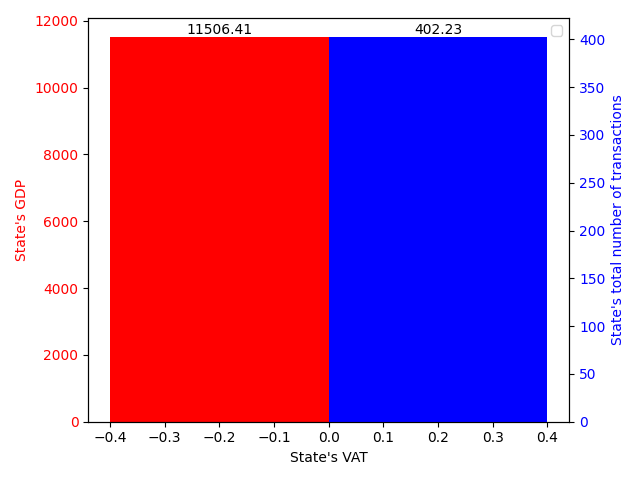
\includegraphics[width=\linewidth]{img/exp/1_2_1.png}
                \caption{No taxes (e.g. VAT of 0)}
            \endminipage\hfill
        \end{figure}

        \subsubsection{Gini coefficient} 
        
        Another interesting metric is the measure of inequalities, i.e. the Gini coefficient, the smaller it is, the more equal a society is. We can, naturally, see a tremendous difference between the two plots. Indeed, if the State has no taxes, it cannot collect nor distribute money. Therefore, the Gini coefficient skyrockets from $0.39$ to $0.96$.

        \begin{figure}[H]
            \minipage{0.5\textwidth}
                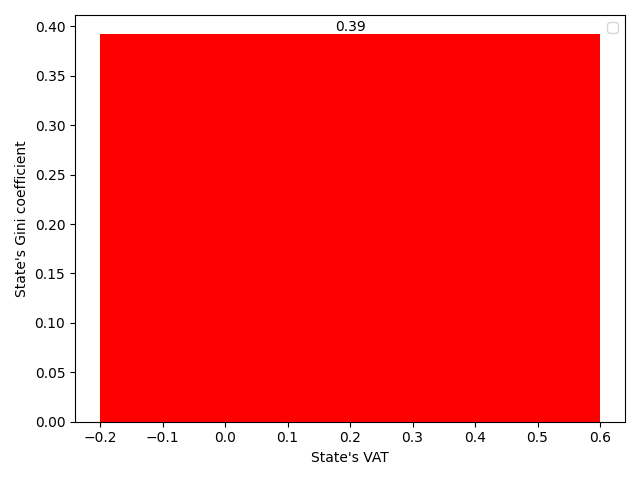
\includegraphics[width=\linewidth]{img/exp/1_1_3.png}
                \caption{Normal taxes (e.g. VAT of 0.2)}
            \endminipage\hfill
            \minipage{0.5\textwidth}
                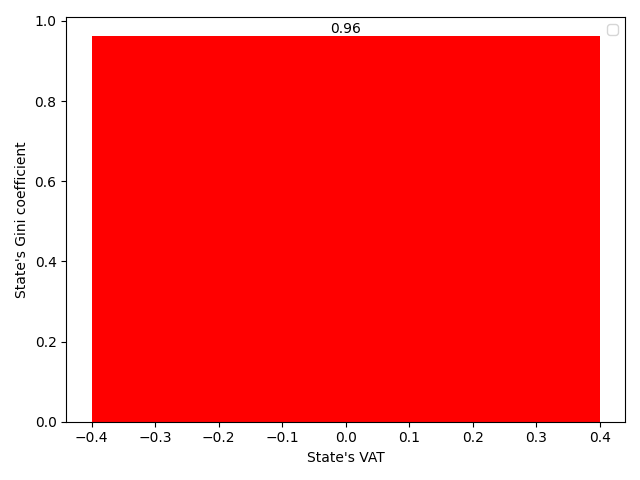
\includegraphics[width=\linewidth]{img/exp/1_2_3.png}
                \caption{No taxes (e.g. VAT of 0)}
            \endminipage\hfill
        \end{figure}

        This experiment shows the importance of having taxes (in the broadest sense of the term) on several metrics in order for our society to advance and be more fair.

    \subsection{Experiment 2: VAT}\label{section:expVAT}
    We will now, for each of the four taxes that were presented, analyze their influence. First: the VAT. For this, we will generate many States with random values for the VAT (ranging from 0 to 1) and see if we can see any pattern emerging regarding some metrics.

        \subsubsection{State GDP and number of transactions}

        \begin{wrapfigure}{l}{0.5\linewidth}
            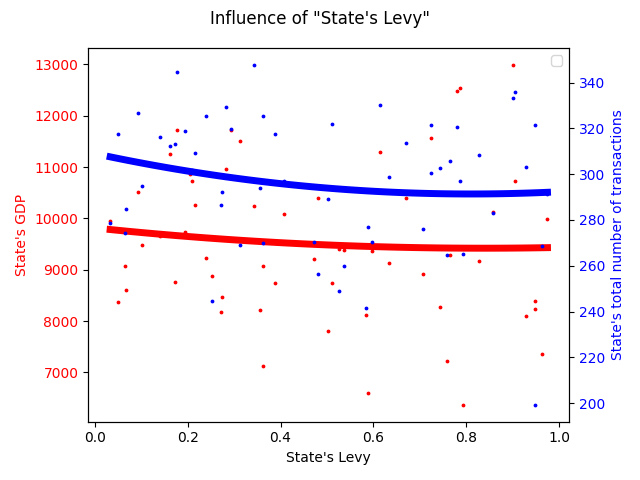
\includegraphics[width=\linewidth]{img/exp/2_1.png}
        \end{wrapfigure} 
        { At first, it is quite surprising to obtain such a plot where no correlation or pattern can be observed. Nonetheless, this makes sense because no matter what the VAT level is, agents will always be able to buy the same amount of products since the money collected from the taxes is always redistributed. For instance, if we have a VAT of 0, our agents will still be able to buy products because States have other taxes to collect money that they will redistribute afterwards. On the other side, if we have a VAT of 1, the State will have more money to redistribute, therefore agents will be richer. They could potentially buy more products, however this will not be the case because of such a high VAT rate making products more expensive.
        \par

        \subsubsection{Gini coefficient}

        \begin{wrapfigure}{r}{0.5\linewidth}
            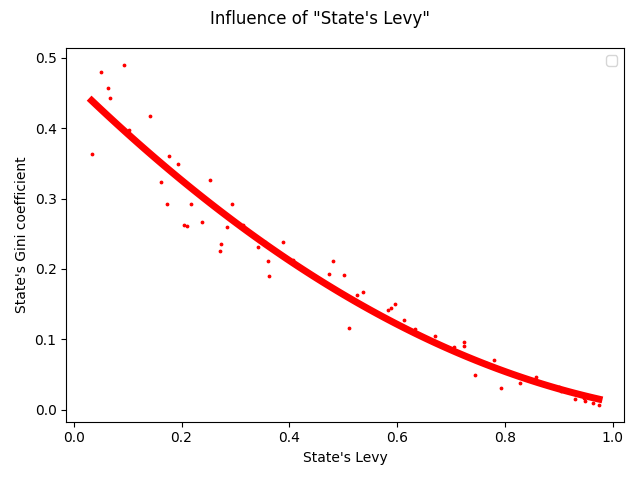
\includegraphics[width=\linewidth]{img/exp/2_3.png}
        \end{wrapfigure} 
        { \lipsum[1-2] Naturally, as we had seen before, the lower the VAT is, the more inequalities we will have since the State has less money to redistribute fairly. However, we can see that here, with a VAT of 0, the Gini coefficient is around 0.45 whereas it was at 0.91 before. This is because in this case, the other taxes are still present as shown in the default configuration allowing the State to distribute allowances and diminishing inequalities. Hence why the higher the VAT is, the less inequalities we have since the Gini coefficient tends to go to zero.
        \par

    \subsection{Experiment 3: Tariff}
    As for the VAT, we will now analyze the influence of the tariff tax by generating many States with random values (ranging from 0 to 1) and see if we can see any pattern emerging regarding some metrics. 

        \begin{figure}[H]
            \minipage{0.5\textwidth}
                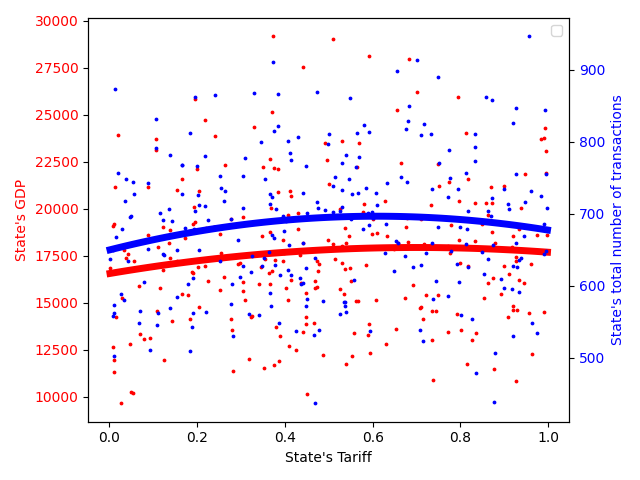
\includegraphics[width=\linewidth]{img/exp/3_1.png}
                \caption{State GDP and number of transactions}
            \endminipage\hfill
            \minipage{0.5\textwidth}
                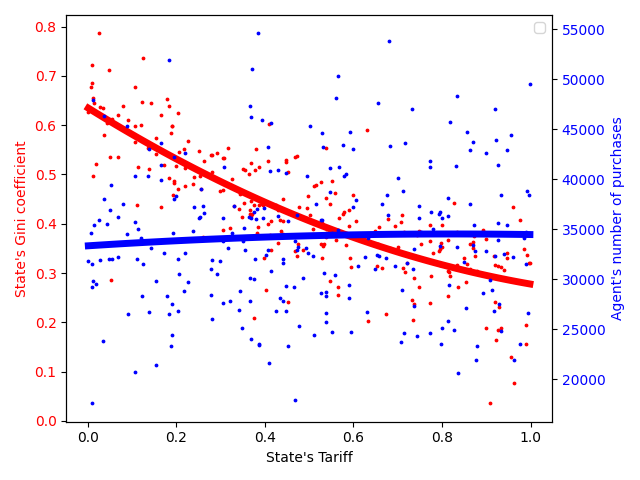
\includegraphics[width=\linewidth]{img/exp/3_3.png}
                \caption{Gini coefficient}
            \endminipage\hfill
        \end{figure}

        As for the previous experiment, the first plot might seem astonishing at first, but the explanation is exactly the same as for the previous experiment~\ref{section:expVAT}. The same goes for the second plot and the analysis of the Gini coefficient.


    \subsection{Experiment 4: Levy}\label{exp:levy}
    We will now analyze the influence of the levy tax by generating many States with random values (ranging from 0 to 1) and see if we can see any pattern emerging regarding some metrics. 

        \begin{figure}[H]
            \minipage{0.5\textwidth}
                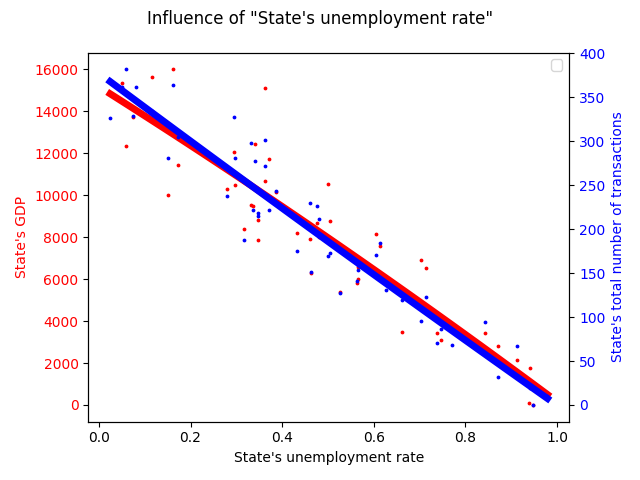
\includegraphics[width=\linewidth]{img/exp/4_1.png}
                \caption{State GDP and number of transactions}
            \endminipage\hfill
            \minipage{0.5\textwidth}
                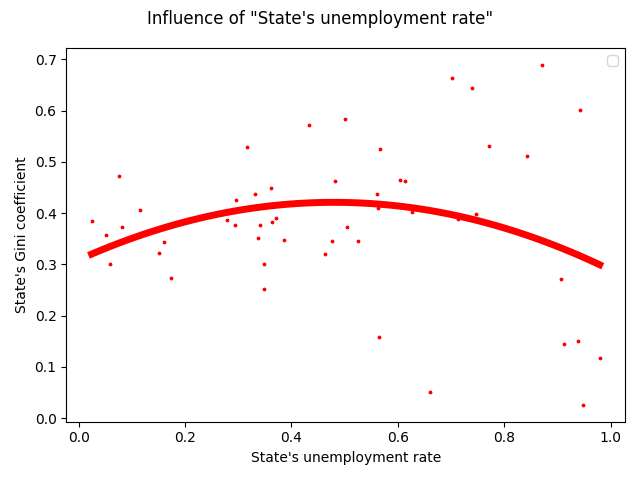
\includegraphics[width=\linewidth]{img/exp/4_3.png}
                \caption{Gini coefficient}
            \endminipage\hfill
        \end{figure}

        As for the previous experiments, the first plot might seem astonishing at first, but the explanation is exactly the same as for the previous experiment~\ref{section:expVAT}. The same goes for the second plot and the analysis of the Gini coefficient. However, in this experiment, the Gini coefficient goes down until almost zero. This was to be expected because if we levy 100\% of the wealth of all agents, they will be moneyless. Therefore, after redistributing the allowances, they will all have the money. Indeed, the Fair and Flat allowance will be almost exactly the same since all agents have the same wealth: none.

    \subsection{Experiment 5: Wealth tax}
    We will now analyze the influence of the last tax: the wealth tax with the same methodologies as the previous taxes and see if we can see any pattern emerging regarding some metrics. 

        \begin{figure}[H]
            \minipage{0.5\textwidth}
                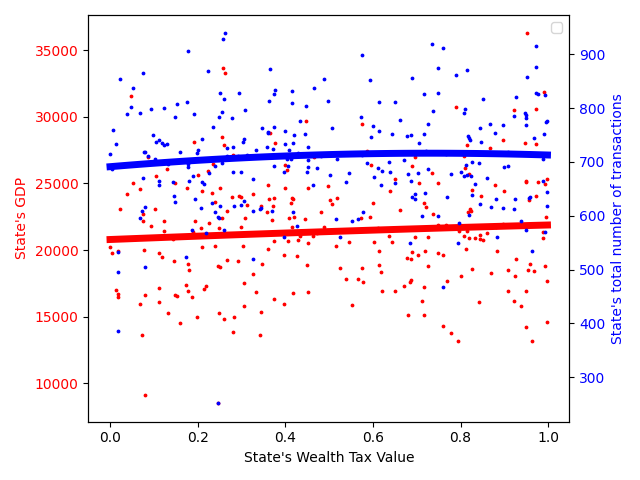
\includegraphics[width=\linewidth]{img/exp/5_1.png}
                \caption{State GDP and number of transactions}
            \endminipage\hfill
            \minipage{0.5\textwidth}
                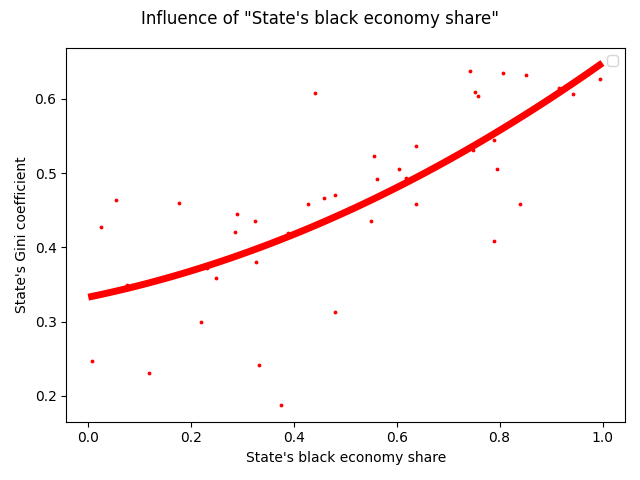
\includegraphics[width=\linewidth]{img/exp/5_3.png}
                \caption{Gini coefficient}
            \endminipage\hfill
        \end{figure}

        As for the previous experiments, the first plot might seem astonishing at first, but the explanation is exactly the same as for the previous experiment~\ref{section:expVAT}. The same goes for the second plot and the analysis of the Gini coefficient.


    \subsection{Experiment 6: Unemployment}\label{exp:unemployment}
    After analyzing the different taxes, we will now focus on another parameter which cannot directly be controlled by the State. As usual, we will create many States with different unemployment rates and see how our metrics change.

            
        \subsubsection{State GDP and number of transactions}

        \begin{wrapfigure}{l}{0.5\linewidth}
            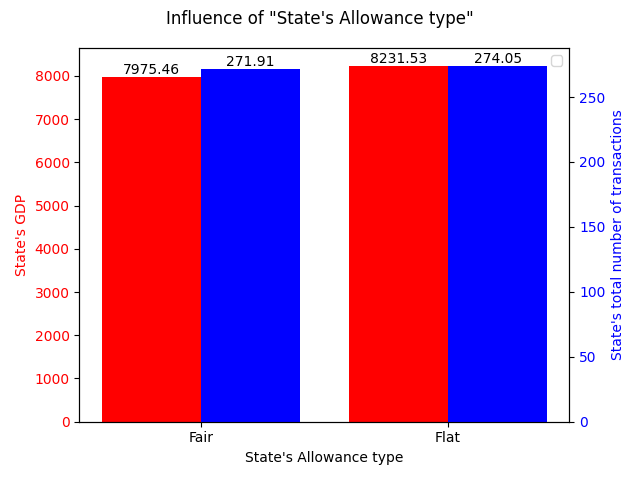
\includegraphics[width=\linewidth]{img/exp/6_1.png}
        \end{wrapfigure} 
        {As one could have expected, we have a rather clear linear correlation. Indeed, the higher the unemployment rate is, the less number of transactions we have and the lower the GDP is. Actually, it is a vicious cycle because the less producers we have, the less products are available on the market, thus less transactions. By having less transactions, we collect less taxes, and therefore do not distribute as much, this means that some agents will never be able to buy another product. 
        \par

        \subsubsection{Gini coefficient}

        \begin{wrapfigure}{r}{0.5\linewidth}
            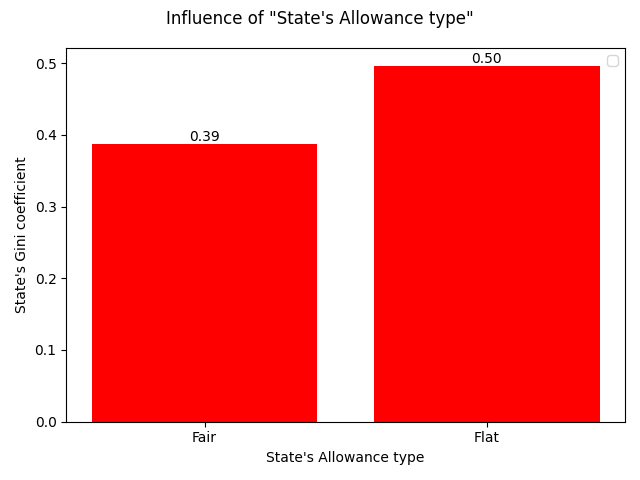
\includegraphics[width=\linewidth]{img/exp/6_3.png}
        \end{wrapfigure} 
        {The plot on the side is a bit tricky but more interesting to analyze. If we only look at the scattered points, we see that there is a linear correlation from the rate 0.0 until 0.8: the more non-producing agents we have, the bigger the Gini coefficient is. This is logical because producing agents will still be able to sell their products and make some money thus accumulating more wealth compared to others, increasing the inequalities.

        However, after the 0.8 rate on the $x$ axis, we can see a significant drop, and the previous statement does not hold true anymore: the Gini coefficient gets very close to zero, i.e. perfect equality. Actually, it also makes sense because if almost everybody is unemployed, then no one can afford to buy any product, thus we have almost no transactions happening and no money flowing between agents, and no agent can therefore become richer than others.
        \par


    \subsection{Experiment 7: Black economy}\label{exp:black}
    The second parameter which cannot directly be controlled by the State is the black economy. As usual, we will create many States with different share of black economy happening and see how our metrics change.

            
        \subsubsection{State GDP and number of transactions}

        \begin{wrapfigure}{l}{0.5\linewidth}
            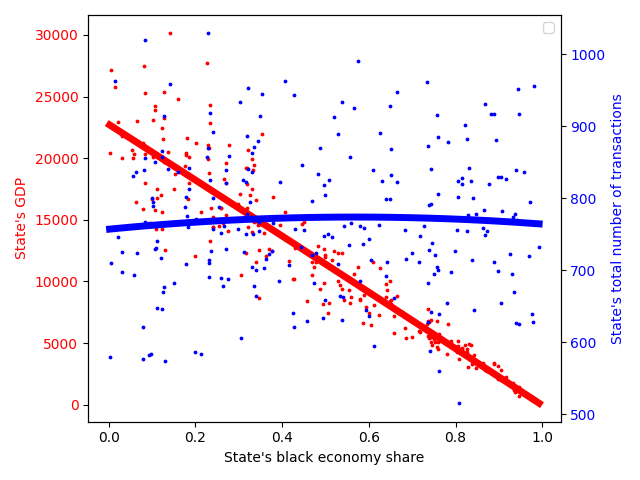
\includegraphics[width=\linewidth]{img/exp/7_1.png}
        \end{wrapfigure} 
        {Until now, we were used to see a strong relation between the number of transactions and the State's GDP. However, this is not the case anymore because of the black economy (because even when no due tax is paid, the transaction is still counted). This results in a linear correlation between the black economy share and the GDP as expected, yet we see absolutely no correlation with the number of transactions since the blue line is quite straight.
        \par

        \subsubsection{Gini coefficient}

        \begin{wrapfigure}{r}{0.5\linewidth}
            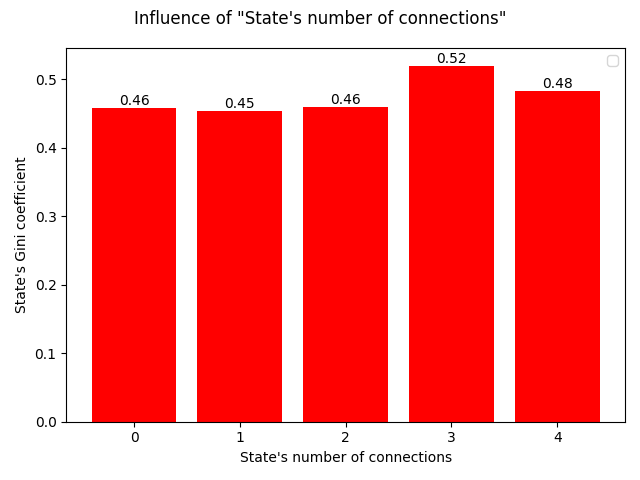
\includegraphics[width=\linewidth]{img/exp/7_3.png}
        \end{wrapfigure} 
        {As the black economy share increases, the inequalities augment as well. This is simply due to the fact that the State will have less money to redistribute when giving allowances, therefore inequalities will subsist even after the small amount of money collected as been redistributed. \\ \\
        \par
    


    \subsection{Experiment 8: Allowances}\label{exp:allowances}
    As we have seen, we have two types of allowances: the flat one (which mimics the Universal Basic Income in the sense that the money is distributed regardless of the agent's wealth), and the fair one (based on the agent's wealth). We will analyze the effects of these two types of redistribution mechanisms.
    
        \subsubsection{State GDP and number of transactions}

        \begin{wrapfigure}{l}{0.5\linewidth}
            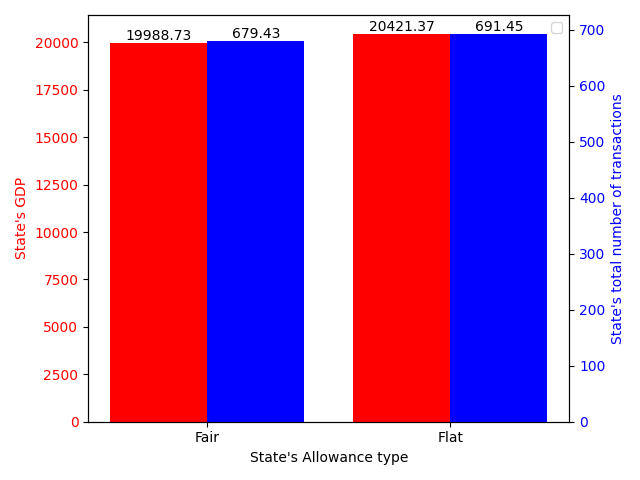
\includegraphics[width=\linewidth]{img/exp/8_1.png}
        \end{wrapfigure} 
        { On this side plot, we see that the flat redistribution mechanism seems to be \emph{slightly} superior to the fair one. The increase is of about $2\%$ (2.1\% for the GDP going from $19988$ to $20421$ and $1.7\%$ for the number of transactions going from 679 to 691). This increase is rather negligible and might be the result of the stochastic behavior of the simulation. Indeed, one would expect to not be a relevant difference on these metrics. For instance, the number of transactions is not penalized by the Flat allowance because poorer agents will still be able to afford buying products since they receive their (equal) share of the total money distributed: all Agents are still able to buy products,.
        \par

        \subsubsection{Gini coefficient}

        \begin{wrapfigure}{r}{0.5\linewidth}
            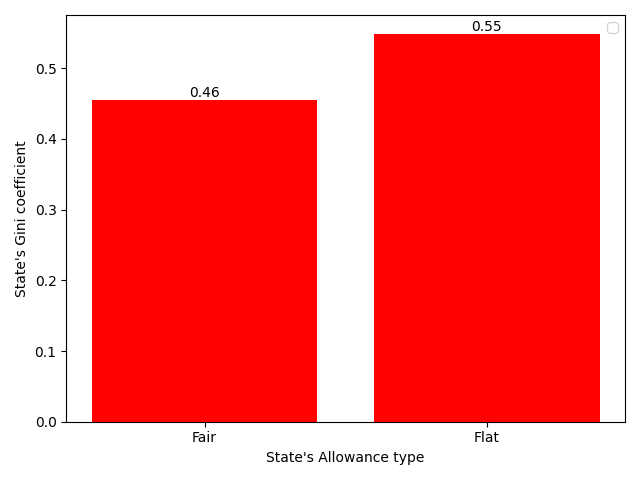
\includegraphics[width=\linewidth]{img/exp/8_3.png}
        \end{wrapfigure} 
        { On the contrary, one would expect a quite pertinent difference on the metric of inequalities as depicted on the plot. This results seems logical since it is was the \emph{main goal} of this redistribution system: State distributing the collected money in a fair way have, in average, a smaller Gini index (i.e. inequalities are limited) and vice-versa for the flat distribution mechanism. With this flat allowance, the wealthier agents will stay wealthier.

        However, an important note to make is that both these systems clearly outperform the system where no redistribution is in place. Indeed, we had seen in the first experiment that, in this case, the Gini coefficient would skyrocket to $0.96$.
        \par



    \subsection{Experiment 9: Connections}
    The final parameter of States that will be analyzed is the number of Connections it has. For this we will study both the bilateral connections and the cluster and their influence on our already well presented metrics. In this experiment, we have a probability of connection of 0.3 and a cluster of 5 States (thus each State is connected to 4 others).

        \subsubsection{State GDP and number of transactions}

        \begin{wrapfigure}{l}{0.5\linewidth}
            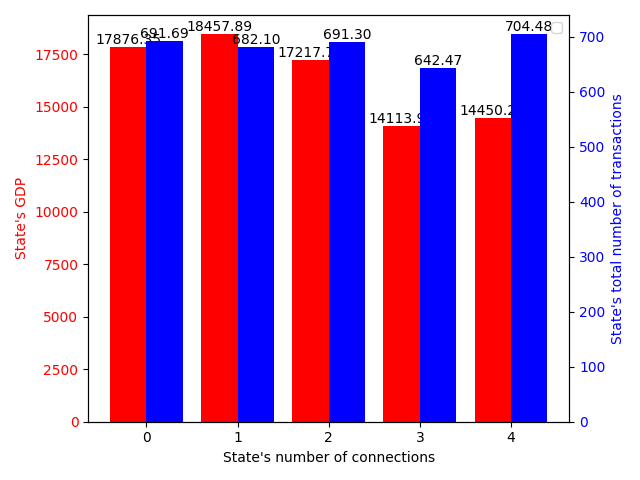
\includegraphics[width=\linewidth]{img/exp/9_1.png}
        \end{wrapfigure} 
        { First, as the number of connected states increases, it seems that the average GDP of these states decreases. Although this may seem odd at first, it fits with our implementation because agents will tend to buy cheaper products since they have a wider range of choices. On the other side, the number of transactions remains quite constant (besides the small drop when a State is connected to 3 others which might be due to the fact that not many States have 3 connections and therefore the statistical relevance is biased).

        With these metrics going towards opposite directions, we can notice something very interesting: the difference between the red (GDP) and blue (number of transactions) bars keeps increasing. Indeed, at first, when a State is connected to no other State, these two metrics are very related as we have seen up until now (besides in the black economy experiment). However, the difference is much more noticeable when a State is connected to 4 other States. The main hypothesis for this behavior is that agents perform as many transactions as before, however because they have access to other markets without any tariffs, they are able to buy some products at a cheaper price in another State therefore not increasing the GDP as much.

        The results of this experiment are quite lackluster when compared to the state of the art. Indeed, an increase of the GDP was expected for State with more connections. This difference is due to the code implementation which does not mimic well enough the reality, and not to the simulation itself. The simulation results fit the implementation.
        \par

        \subsubsection{Gini coefficient}

        \begin{wrapfigure}{r}{0.5\linewidth}
            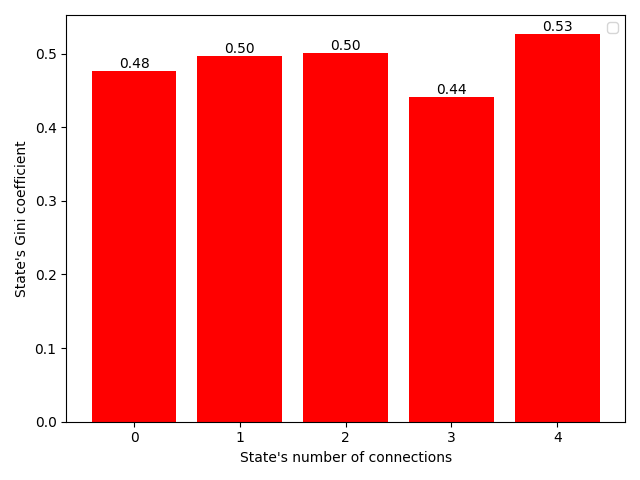
\includegraphics[width=\linewidth]{img/exp/9_3.png} 
        \end{wrapfigure}   
        { Regarding the measure of inequalities, we see that all the Gini coefficients are very similar to one another. The differences are quite negligible when compared to the others when had before (0.46 versus 0.55, or 0.39 versus 0.96). Having access to a larger market with cheaper prices does not, in fine, mean that inequalities will be reduced/accentuated for those agents since both the wealthiest and the poorest agents will buy these cheaper products, therefore no reduction of difference of wealth was expected. 
        \par
    

    \subsection{Experiment 10: Number of ticks}
        
        \begin{wrapfigure}{l}{0.5\linewidth}
            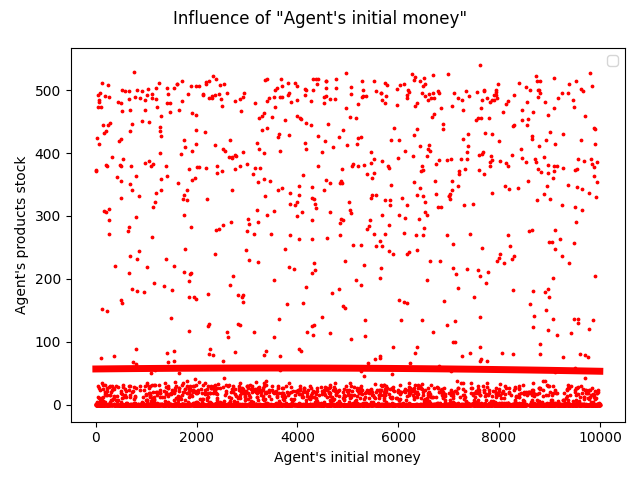
\includegraphics[width=\linewidth]{img/exp/10_2.png}
        \end{wrapfigure} 
        { Our last experiment of this section is not based on a parameter of the state \emph{per se}, but on the duration of the simulation and the evolution of some State metrics as the number of ticks increases. Deciding how long the simulation should run for is important to save computational power and run-time by checking at around how many ticks the simulation starts to stabilize. After this point of stabilization, there is no real advantage of running the simulation for even longer because no dramatic fluctuation should happen. 
            
        As we can see on this plot, the simulation metrics start to stabilize after 2000 or 3000 ticks and going up to 6000 ticks provides no advantage (for a run-time 2-3 times longer). Hence, the default number of ticks in the configuration file is 3000.
        \par
    
\section{Agent experiments}
    After seeing and analyzing some State parameters, we will focus on those of the Agents.

    \subsection{Experiment 11: Talent}
    The talent an agent has lets it produce cheaper products therefore having more chances at getting picked by a potential buyer looking for the cheapest product. For this experiment, we will analyze how the talent of an agent (between 0 and 1) influences its sales and purchases by generating lots of homogeneous agents with different talent values.

        \begin{wrapfigure}{r}{0.5\linewidth}
            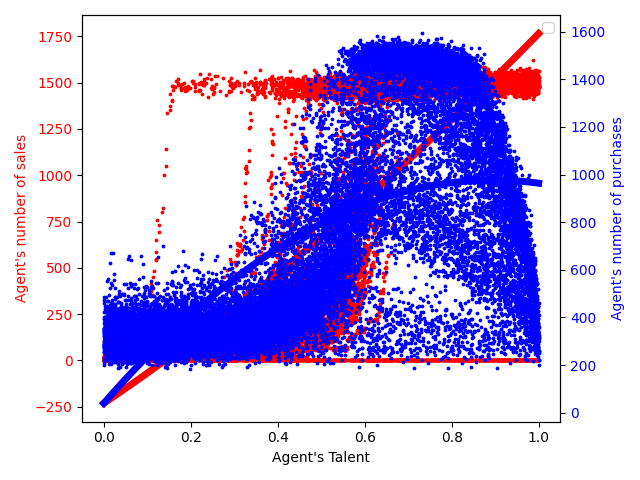
\includegraphics[width=\linewidth]{img/exp/11.png}
        \end{wrapfigure} 
        { This first plot may look quite chaotic and random at first, however we can see many interesting patterns by taking into account some particularities afterwards. First, generally we see a trend (red line behind the blue dots) that the more talent an agent has, the more sales it will make. Regarding the number of purchases, we have a rather odd pattern (which looks like the on in the Gini coefficient in the Unemployment experiment): as the talent increases, we are gradually able to make more purchases until a certain point around 0.5-0.7. After this point, there is a significant drop due to the fact that agents will produce products ``too cheap'', therefore not allowing them to earn enough wealth and make purchases. This is quite interesting because it shows that selling at such low prices is not always a good idea.
        
        However, it seems that the trends are not linear (as one could have expected) but this due to the fact a different products have different base prices (i.e. the original price of the product which is then lowered by a certain factor based on the agent's talent). For instance, if we have an agent A which produces a product with a base price of 10 with a talent of 0.1, then A will see its product at 9. Now if we have another agent B which produces a product with a base price of 200 with a talent of 0.7, its product will now cost 60. This means that, even though A has less talent (0.1) than B (0.7), it will \emph{probably} sell more products since its product remains cheaper, therefore we do not have a clear linear trend.
        This is also the reason why we a trace of red scattered points going upwards: the same product: the point goes up (i.e. more sales) as the talent goes up too.

        \par


    \subsection{Experiment 12: Initial money}
    Another interesting parameter is the initial money of an agent. Whether an agent starts the simulation with a small or huge amount of money could influence its purchases and sales. 

        \begin{wrapfigure}{l}{0.5\linewidth}
            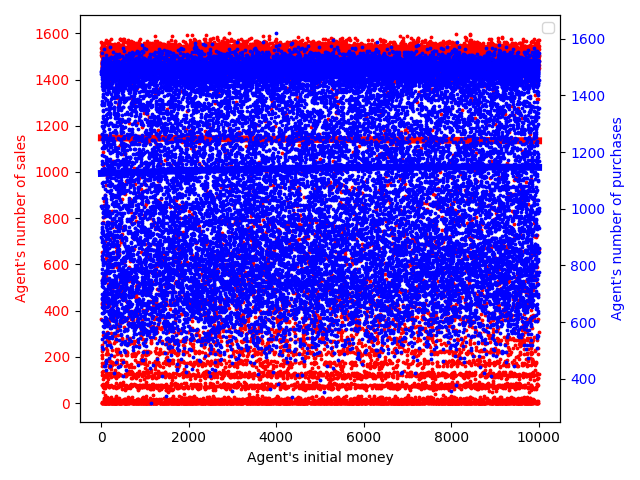
\includegraphics[width=\linewidth]{img/exp/12_1.png}
        \end{wrapfigure} 
        { Again, the plot looks a bit chaotic because of the many points (i.e. agents). However, we can clearly see that there is absolutely no correlation between the agent's initial money and its sales or purchases (both the blue and red lines are horizontal and the scattered points are very sparse across the plot). This was to be expected because of the redistribution. Indeed, although an agent may start with little money, it will still be able to make purchases with the money it receives from its sales and from the allowances it will receive during the simulation. 
        \par



    \subsection{Experiment 13: Unemployment}
    As we had seen in a previous experiment, unemployment (i.e. agent who never produces) plays a major role in the System. How can agents who do not produce make purchases ? For this experiment we will only have one State with a thousands agents and un employment rate of 0.3. To see the role of unemployment, we will compare one simulation which runs for 1000 ticks, and another for 10000 ticks.

        \begin{figure}[H]
            \minipage{0.5\textwidth}
                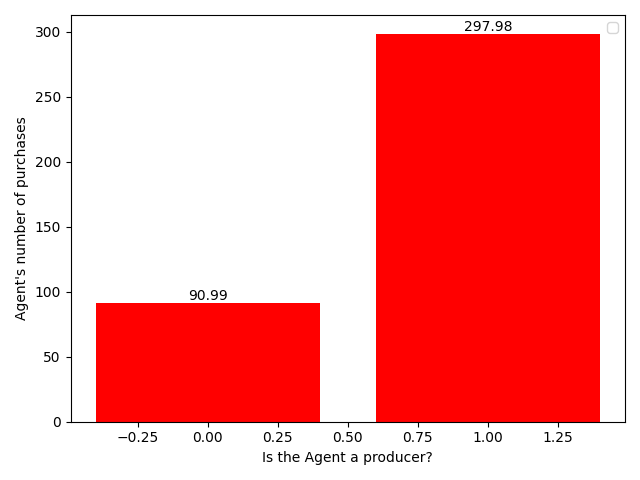
\includegraphics[width=\linewidth]{img/exp/13_1.png}
                \caption{1000 ticks}
            \endminipage\hfill
            \minipage{0.5\textwidth}
                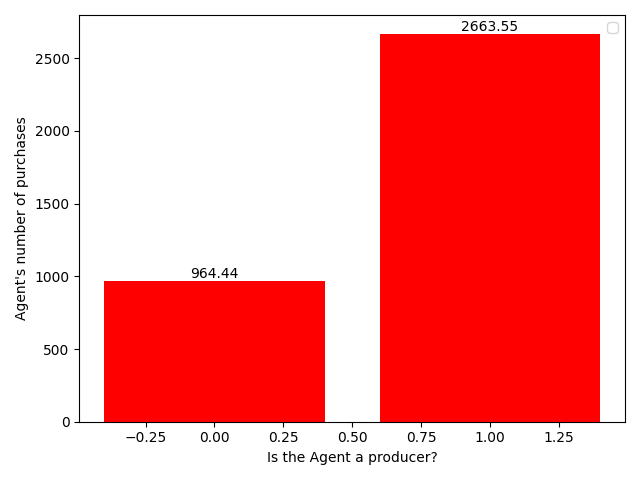
\includegraphics[width=\linewidth]{img/exp/13_2.png}
                \caption{10000 ticks}
            \endminipage\hfill
        \end{figure}

    As we can see on these plots (where 1 means that the agent is indeed a producer, and 0 means it is unemployed). Naturally, producers make more purchases than non-producers (2.2x times as much for 1000 ticks and 1.7x as much for 10000 ticks). However, we can see that in both cases, multiplying by 10 the number of ticks results in a \emph{roughly} 10 times increase of the number of purchases for both producers and non producers. This means that  non-producing agents can make purchases thanks to the redistribution system. Indeed, otherwise, if they were no allowances, the non-producing agents would be able to buy products up until a certain point where they have spent all their initial money. From that tick forward, they would not be able to make any purchase because they would not sell anything nor receive any money from the State, therefore a threshold would be reached, and increasing the number of ticks would not upgrade the threshold (contrary to here).
    

    \subsection{Experiment 14: Wealth distribution}
    We can see in the following comparison the difference between the wealth distribution among agents. This wealth distribution is presented by the Lorenz curve (in blue). 

    \begin{figure}[H]
        \minipage{0.5\textwidth}
            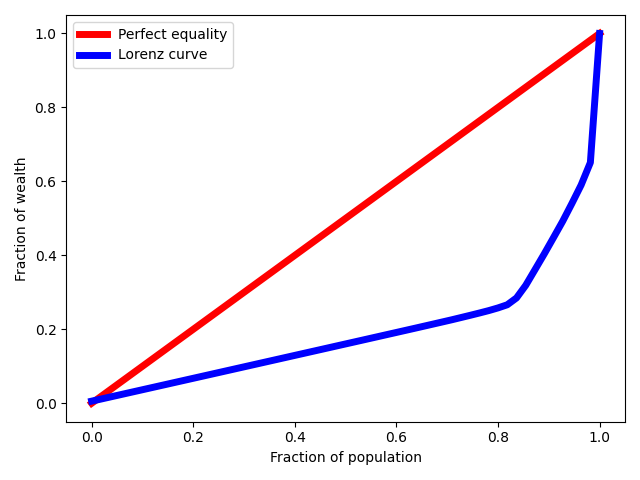
\includegraphics[width=\linewidth]{img/exp/14_1.png}
            \caption{Flat allowance State}
        \endminipage\hfill
        \minipage{0.5\textwidth}
            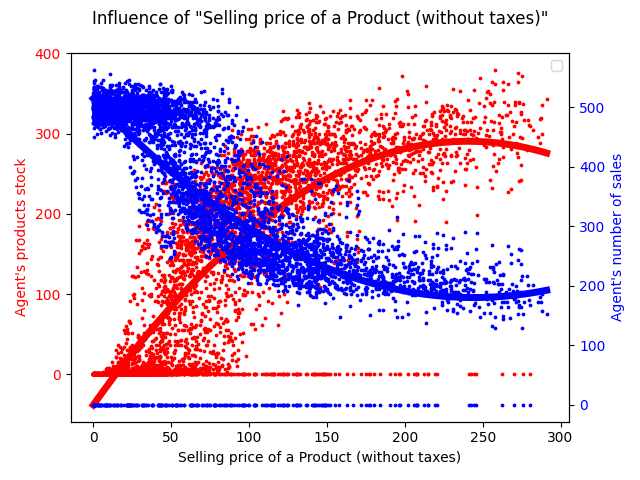
\includegraphics[width=\linewidth]{img/exp/14_2.png}
            \caption{Fair allowance State}
        \endminipage\hfill
    \end{figure}

    We can read this plot as follows: if we take the x point 0.8 in the left hand-side plot, we can see that 80\% of the population owns around 25\% of the total wealth. On the other plot, we see that at 80\% of the population owns around 40\% of the total wealth. Therefore, the second case seems fairer. In a perfect equality society, we would obtain the red curve: 30\% of the population detains 30\% of the wealth, 80\% would own 80\%, etc. 
    
    Therefore, the bigger the area between the red and blue curves, the higher the inequalities will be. This area actually represents one metric that we have analyzed all along this thesis: the Gini coefficient. If both curve coincide, the Gini index will be 0. On the other side, if there is only one person holding all the wealth and all the others agents own nothing, then we would see a blue horizontal line at the bottom with a sudden peak at then end therefore resulting in a Gini coefficient very close to 1. \footnote{Not \emph{exactly} 1 because we would need an infinite amount of agents}.

    The Gini coefficient on the left plot (where a flat allowance redistribution system is used) is equal to 0.618 whereas on the right hand-side the Gini index is equal to 0.546. Naturally, we can see that the right case is fairer as wealth is distributed a bit more fairly.


\section{Product experiments}
    Finally, our last two experiments will be about the products. 


    \subsection{Experiment 15: Selling price}
    

        \begin{wrapfigure}{l}{0.5\linewidth}
            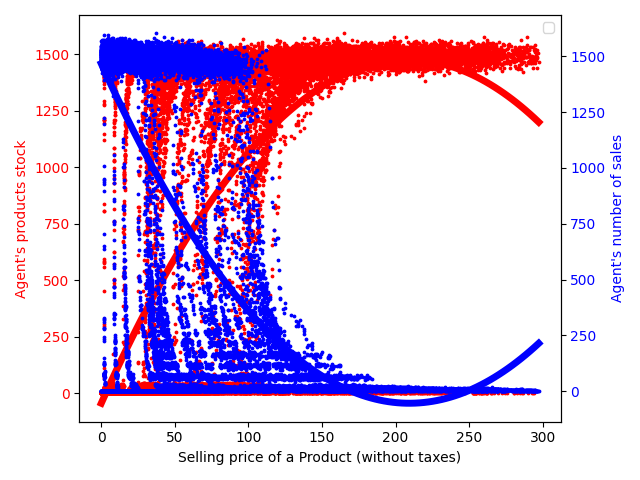
\includegraphics[width=\linewidth]{img/exp/15.png}
        \end{wrapfigure} 
        { The first basic parameter of a product is the selling price. We can analyze its impact on two metrics: the number of stocks remaining, and, of course, the number of sales of that product. Naturally, these two curves metrics are the opposite of each other: more sales means less stocks remaining. We see that the trends are not totally linear. This is because we are analyzing the selling price without any taxes. By adding the VAT and the custom tariffs (if applicable), a cheaper product might become more expensive, therefore resulting in these solitary scattered points. 
        \par


    \subsection{Experiment 16: Choosing method}
    As introduced before, after an agent filters the available products according to their type, price, etc., it should choose one among those possibilities. There are three ways of picking a product: cheapest, random, weighted-random as previously explained. We will analyze these three choosing methods.

    \begin{figure}[H]
        \minipage{0.32\textwidth}
            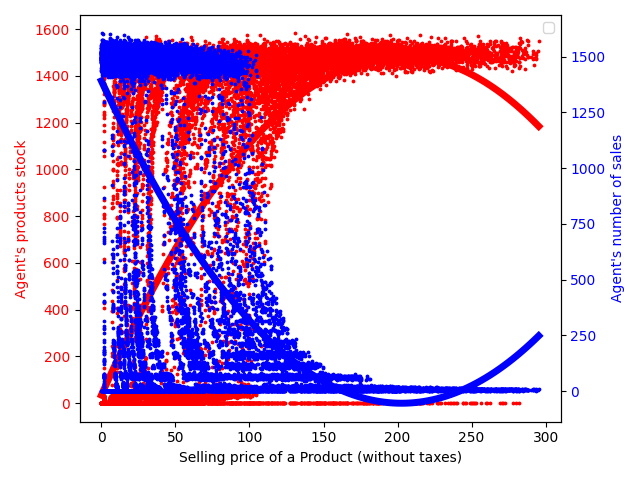
\includegraphics[width=\linewidth]{img/exp/16_1.png}\label{fig:cheapest}
            \caption{Cheapest}
        \endminipage\hfill
        \minipage{0.32\textwidth}
            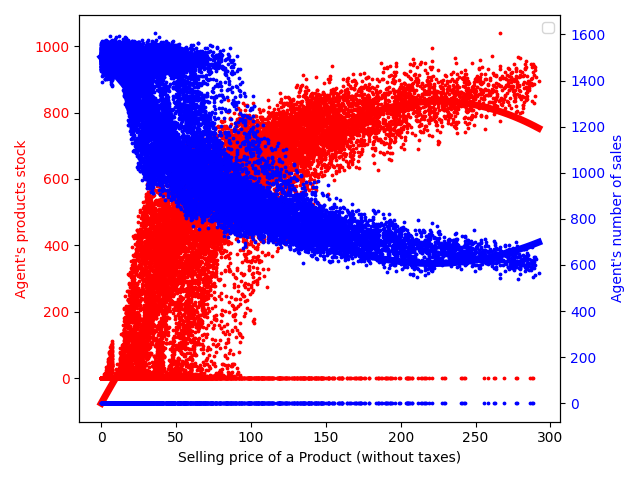
\includegraphics[width=\linewidth]{img/exp/16_2.png}\label{fig:random}
            \caption{Random}
        \endminipage\hfill
        \minipage{0.32\textwidth}
            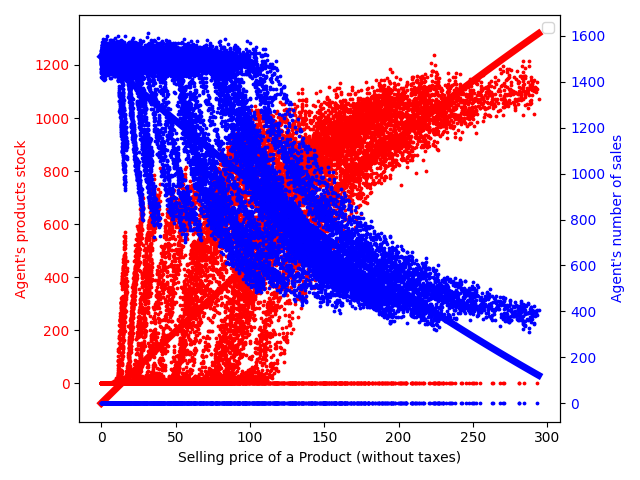
\includegraphics[width=\linewidth]{img/exp/16_3.png}\label{fig:weighted}
            \caption{Random weighted}
        \endminipage\hfill
    \end{figure}

    The first plot has already been analyzed and explained in the previous section (because the default choosing method is 'Cheapest'). We will compare it with other two methods. 
    
    In the middle plot, where a random method is used, we can see that agents will more easily buy more expensive products since we have more scattered points on the right hand-side of the plot (compared to the first plot) as we wanted. Although products are selected at random despite the price, we must recall that we have a filtered list of \emph{possibilities} according to the budget of the agent. Thus, naturally, we have more points on the upper left part of the plot (i.e. small price = more sales) because these products are more frequently in this filtered list, therefore they will be picked more often too compared to expensive products which will get picked less often given the fact that they are not always present in that list. This explains why we do not have a totally horizontal blue line.

    Finally, on the last plot we can see a intermediary result: we see a mix of the two plots in the sense that sometimes we do make a random choice, but it biased towards cheapest possibilities.


\section{Experiments conclusion}
    As we have seen in these experiments, we had different kind of results: some which were quite straightforward and expected, others were very interesting to analyze and finally some were disappointing because they did not match the reality. In the latter case, we hypothesized that it might due to the many details of the real life which are not taken into account here. However, we were able to answer the majority of our research questions presented in the introduction.
